
\chapter{Heat module}

\section{Heat module - Part 1}


%%----------------------------------------------------------------------------------------
%%	INTRODUCTION
%%----------------------------------------------------------------------------------------
\subsection{Goal and Complexity}
\subsubsection*{Complexity: Beginner}

\subsubsection*{Prerequisites: None}

The goal of this tutorial is to get familiar with the $DRUtES$ heat module and  $DRUtES$ configuration in 1D by simulating heat conduction through a 20 cm thick wall.\medskip

\begin{figure}[!h]
\centering
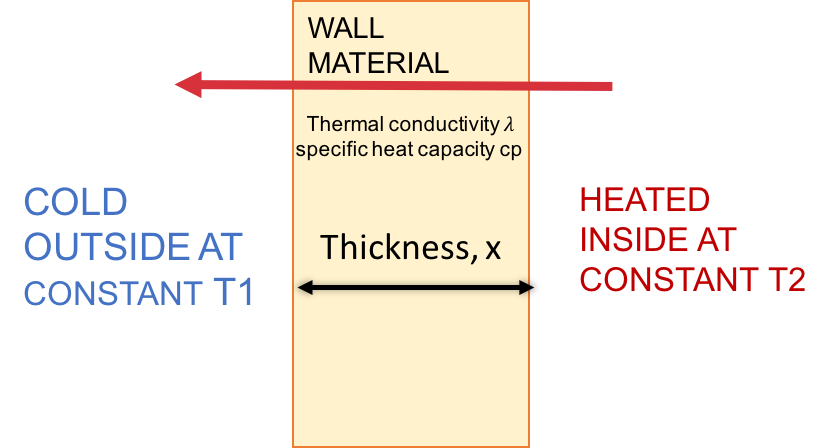
\includegraphics[width=8cm]{Fig_heat1/heat_cond_simple.png}
\end{figure}
Heat flow is important in the soil. To simplify, we're assuming heat flow through a wall. We test different insulation materials by assigning different heat capacities and thermal conductivity values of several real-world materials. 

In this tutorial three configuration files will be modified step by step. All configuration files are located in the folder \emph{drutes.conf} and respective subfolders. \begin{enumerate}
\item For selection of the module, dimension and time information we require \emph{global.conf}.  \emph{global.conf} is located in \emph{drutes.conf / global.conf}. 
\item To define the mesh or spatial discretization in 1D,  we require \emph{drumesh1D.conf}. \emph{drumesh1D.conf} is located in \emph{drutes.conf / mesh / drumesh1D.conf}. 
\item To define heat conduction, we require \emph{heat.conf}. \emph{heat.conf} is located in \emph{drutes.conf / heat / heat.conf}. 
\end{enumerate}
$DRUtES$ works with configuration input file with the file extension .conf. Blank lines and lines starting with \# are ignored. The input mentioned in this tutorial therefore needs to be placed one line below the mentioned keyword, unless stated otherwise. 



\newpage
\subsection{Scenarios}

For all scenarios, we assume that the wall is between a heated room, which is maintaining a constant temperature of 20 $^{\circ}$C, and the outside world during winter, which for the sake of simplicity is at a constant temperature of 0 $^{\circ}$C.
The outside temperature and the heated room temperature are our boundary conditions. They define the limits of our spatial domain. They give us a lot of information on our problem. We already know the solution of our problem at the boundaries and they do not change over time. This type of boundary condition is called \textbf{Dirichlet boundary condition}. 
We assume 1D flow. This means that we are only interested in one-direction. Although this might seem drastic, it only means that the other directions are homogeneous and do not provide us with more information.

We can assume a simple domain set-up as in Fig. \ref{dsuh1}. What is missing is the material properties defining the heat conduction. These can be found in Tab. \ref{tab_heat} for three different materials: stone concrete, sand stone and cotton.

\begin{figure}[!h]
	\centering
	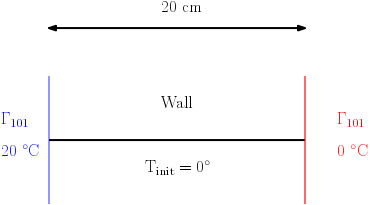
\includegraphics[width=0.6\textwidth]{Fig_heat1/domain_setup_h1.png}
	\caption{\label{dsuh1} Domain set-up for 1D heat conduction through a wall with two constant Dirichlet conditions.}
\end{figure} 

\begin{table}[!h]\caption{\label{tab_heat}Material properties needed for scenarios.}
	\centering
\adjustbox{max height=\dimexpr\textheight-5cm\relax,
           max width=\textwidth}{

\small\begin{tabular}{l c c c}
\hline
& specific heat capacity & density & thermal conductivity\\
& c$_p$ &  $\rho$ & $\lambda$ \\
Material & [J kg$^{-1}$ K$^{-1}$] & [kg m$^{-3}$] & [W m$^{-1}$ K$^{-1}$  ] \\
 \hline
Stone concrete & 750 & 1400 & 1.7 \\
Sand stone & 920 & 2800 & 1.7 \\
Cotton &  1340& 1550 &0.04 \\
\hline
\end{tabular}
}
\end{table}



\section*{Scenario 1}

Heat conduction through a 20 cm thick stone concrete wall. 

$global.conf$: Choose correct model, dimension, time discretization and observation times.
\begin{enumerate}
\item Open \textbf{\emph{global.conf}} in a text editor of your choice. 
\item Model type: Your first input is the module. Input is \textbf{heat}.
\item Initial mesh configuration \begin{enumerate}
\item The dimension of our problem is 1. Input: 1.
\item We use the internal mesh generator. Input: 1. 
\end{enumerate}
\item Error criterion (not needed here, leave at default value) \begin{enumerate} 
\item Maximum number of iteration of the Picard method: 20 
\item h tolerance: 1e-2.
\end{enumerate}
\item Time information 
\begin{enumerate} 
%\item integration method is 3 point formula. Input: 30. 
\item Time units are in hours: input h
\item Initial time: 1e-3.
\item End time: 24.
\item Minimum time step: 1e-6.
\item Maximum time step: 0.1.
\end{enumerate}
\item Observation time settings \begin{enumerate}
\item Observation time method: 2
\item Set file format of observation: pure. Output in 1D is always in raw data. Different options will not impact output in 1D.
\item Make sequence of observation time: n
\item Number of observation times: 11
\item Observation time values: 2, 4, 6, 8, 10, 12 ,14, 16, 18, 20, 22. Use a new line for each input. \textit{DRUtES} automatically generates output for the initial time and final time. DRUtES will generate 13 output files, e.g. \textit{heat\_temperature-x.dat}, where x is the number of the file and not the output time. The initial time is assigned an x value of 0. 
\end{enumerate}
\item Observation point settings \begin{enumerate}
\item Observation point coordinates: 0.0, 0.2. Use a new line for each input. \textit{DRUtES} will generate 2 output files, e.g. \textit{obspt\_heat-x.out}, where x is the ID of the observation point. 
\end{enumerate}
\item Ignore other settings for now. 
\item \textbf{Save $global.conf$}!!!
\end{enumerate}


$drumesh1D.conf$: Mesh definition, i.e. number of materials and spatial discretization
\begin{enumerate}
\item Open \textbf{\emph{drumesh1D.conf}} in a text editor of your choice. 
\item Geometry information: 0.2 m - domain length
\item Amount of intervals: 1
\item
\adjustbox{max height=\dimexpr\textheight-5cm\relax,
           max width=\textwidth}{
\small\begin{tabular}{|c | c | c|}
\hline
density & bottom & top \\
 \hline
0.005 & 0 & 0.2 \\
\hline
\end{tabular}
}
\item number of materials: 1
\item \adjustbox{max height=\dimexpr\textheight-5cm\relax,
           max width=\textwidth}{
\small\begin{tabular}{|c | c | c|}
\hline
id & bottom & top \\
 \hline
1& 0 & 0.2 \\
\hline
\end{tabular}
}
\end{enumerate}

\emph{heat.conf}: Heat module after Sophocleous (1979). 


\begin{enumerate}
\item Open \emph{heat.conf} in a text editor of your choice. 

\item Couple with Richards equation: n
\item Number of materials or layers: 1 
\item Specific heat capacity of the wall material: \\750 J kg$^{-1}$ K$^{-1}$ x 1400 kg m$^{-3}$ = 1.05E6 J m$^{-3}$ K$^{-1}$ = $\frac{1.05E6~\mathrm{W~s~m^{-3}~K^{-1}}}{3600~\mathrm{s~h^{-1}}}$ \\= 291 W h m$^{-3}$ K$^{-1}$. 
\item Specific heat capacity of liquid: 0
\item Anisotropy: There is no anisotropy. The value is 0.
\item Heat conductivity of the wall material: 1.7 W m$^{-1}$ K$^{-1}$. 
\item There is NO heat convection of water: 0.
\item The initial temperature is 0$^{\circ}$C across the entire domain: 0.
\item There is no heat source: 0. 
\item We have 2 boundaries at both ends of the wall. We assume a constant temperature of 0 $^{\circ}$C outside. We assume the inside is heated and the temperature maintained at exactly 20$^{\circ}$C. We therefore know the temperature at the boundaries. We also know that these values do not change in time. They can be describes as time-constant Dirichlet boundary conditions. \\
\adjustbox{max height=\dimexpr\textheight-5cm\relax,
           max width=\textwidth}{
\small\begin{tabular}{|c | c | c| c|}
\hline
boundary id & boundary type & use bc.dat & value \\
 \hline
101& 1 & n & 20.0 \\
102& 1 & n & 0.0 \\
\hline
\end{tabular}
}

\item Save heat.conf.
\end{enumerate}

\section*{Run scenario 1}
Run the simulation in the terminal console.
\begin{enumerate}
\item Make sure you are in the right directory. 
\item To execute $DRUtES$: \\
\$ bin/drutes
\item After the simulation finishes, to generate png plots execute provided R script: \\
\$ Rscript drutes.conf/heat/heatplots.R concrete
\item The output of the simulation can be found in the folder out
\end{enumerate}

\section*{Tasks for scenario 1}

\begin{enumerate}
\item How long does it take for the temperature distribution to become linear between the two observation points?
\item How large is the steady state heat flux through the wall?
\item Let's assume a wall area of A=15 m$^2$. Use the observation point at the boundary between the wall and the inside of room. How large was the cumulated heat loss 24 h. How much will be lost after 48 h when the set-up does not change?
\end{enumerate}


\section*{Result of scenario 1}

\subsection*{Question 1}
Figure \ref{plot1} shows that the temperature distribution becomes linear quite quickly and reaches a steady state after observation time 2, which was set to 4 h. Figure \ref{plot2} shows the heat flux $\phi_{\mathrm{p}}$ in observation points 1 (red) and 2 (blue) bordering the wall to the outside and heated inside, respectively.  The heat flux is extremely large at observation point 2 in the beginning. Observation point 2 evidently defines the boundary between the wall and the heated inside. After approximately 3 hours, the heat flux of observation point 1 and 2 become identical. This occurs when the simulation reaches steady state and a linear temperature distribution. Figure \ref{plot2} allows a more exact estimation of when the system becomes steady state. 

\begin{figure}[!h]
\centering
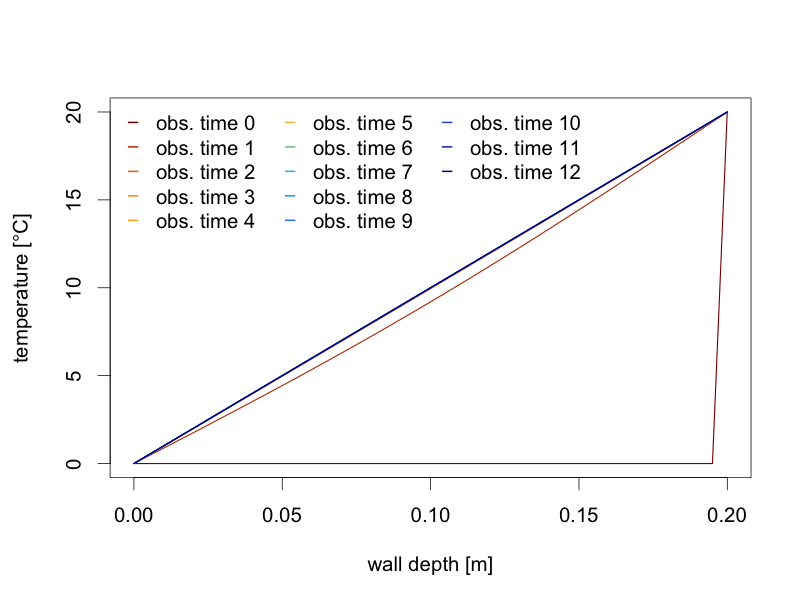
\includegraphics[width=10.5cm]{Fig_heat1/obs_time_temp_concrete.png}
\caption{\label{plot1}Plot of observation times for stone concrete generated with Rscript heatplots.R}
\end{figure}

\subsection*{Question 2}

\begin{figure}[!h]
\centering
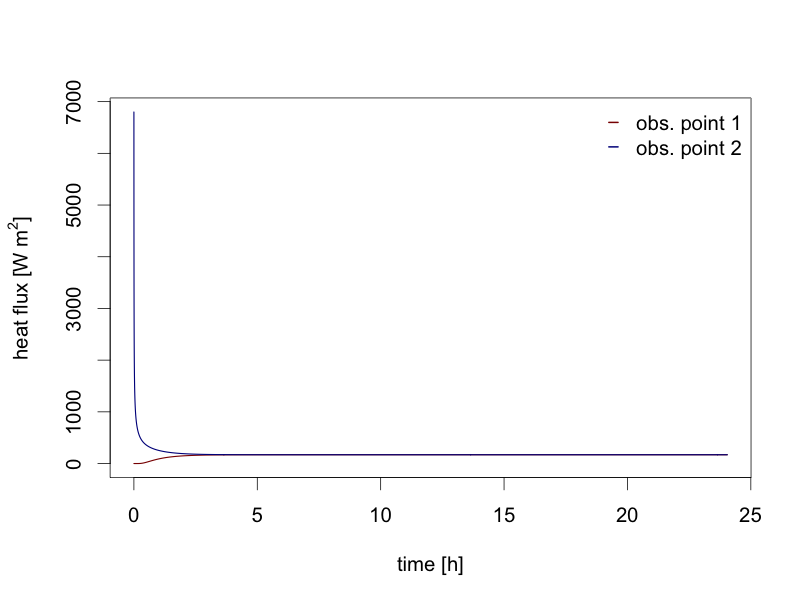
\includegraphics[width=10.5cm]{Fig_heat1/obs_point_temp_concrete.png}
\caption{\label{plot2} Heat flux at observation points 1 and 2 for stone concrete generated with Rscript heatplots.R}
\end{figure}

The constant heat flux value is at $\phi_{p}$=170 W m$^{-2}$. This value can also be calculated using the equation:
\begin{equation*}
\phi_{\mathrm{p}}=-\lambda\frac{dT}{dx}= -1.7 \frac{20-0}{0.2}= 170 \mathrm{~W~m^{-2}}
\end{equation*}

\newpage
\subsection*{Question 3}

Figure \ref{plot3} shows the cumulative heat flux in observation points 1 and 2, both ends of the wall. The cumulative heat flux after 24 h at observation point is 4468 W m$^{-2}$. With a wall area of 15 m$^2$ this results in $Q = 4468~\mathrm{W~h~m^{-2}}\cdot~15~\mathrm{m^{2}}= 67020 ~\mathrm{W~h}$. 
For the next 24 h, the heat flux will be constant at 170 $\mathrm{~W~m^{-2}}$. The total heat loss will therefore be $Q=170 \mathrm{~W~m^{-2}}~\cdot 24~\mathrm{h}~\cdot~15~\mathrm{m^{2}}=61200 \mathrm{~W~h}$.

\begin{figure}[!h]
\centering
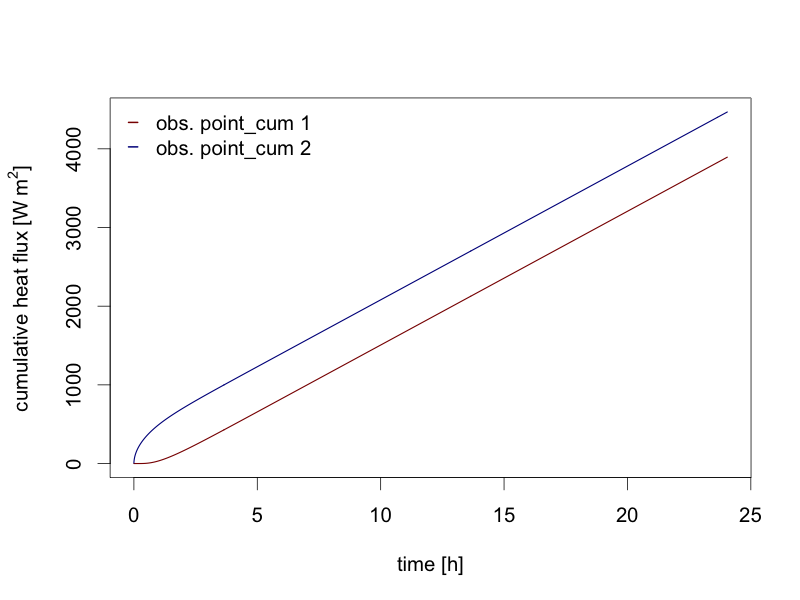
\includegraphics[width=10.5cm]{Fig_heat1/obs_point_cum_temp_concrete.png}
\caption{\label{plot3} Cumulated heat flux at observation points 1 and 2 for stone concrete generated with Rscript heatplots.R}
\end{figure}

\newpage

\section*{Scenario 2}
Heat conduction through a 20 cm thick sandstone wall. 

\begin{enumerate}
\item Open \emph{heat.conf} in a text editor of your choice. 
\item Leave all settings the same, except for specific heat capacity. 
\item Replace the specific heat capacity with values of sand stone.
\item Save heat.conf.
\end{enumerate}

\section*{Run scenario 2}
Run the simulation in the terminal console.
\begin{enumerate}
\item Make sure you are in the right directory. 
\item To execute $DRUtES$: \\
\$ bin/drutes
\item After the simulation finishes, to generate png plots execute provided R script: \\
\$ Rscript drutes.conf/heat/heatplots.R sandstone
\item The output of the simulation can be found in the folder out
\end{enumerate}

\section*{Tasks for scenario 2}

\begin{enumerate}
\item Answer the same questions as for scenario 1. What is different?
\end{enumerate}

\section*{Result of scenario 2}
\subsection*{Question 1}
Figure \ref{plot4} shows that it takes longer for the temperature distribution to become linear in sandstone than in concrete sand. Also taking Fig. \ref{plot5} into account, it takes approximately 5 h. This is because sandstone has a larger specific heat capacity than stone concrete.

\begin{figure}[!h]
\centering
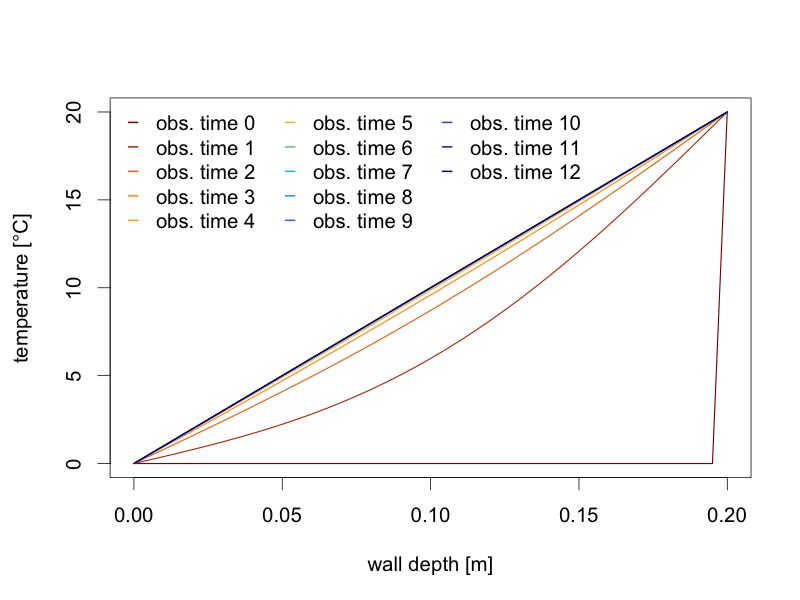
\includegraphics[width=10.5cm]{Fig_heat1/obs_time_temp_sandstone.png}
\caption{\label{plot4}Plot of observation times for sandstone generated with Rscript heatplots.R}
\end{figure}

\subsection*{Question 2}

The constant heat flux when the system is in steady state is also at $\phi_{p}$=170 W m$^{-2}$. Both materials have the same thermal conductivity and therefore the same thermal heat flux.

\begin{figure}[!h]
\centering
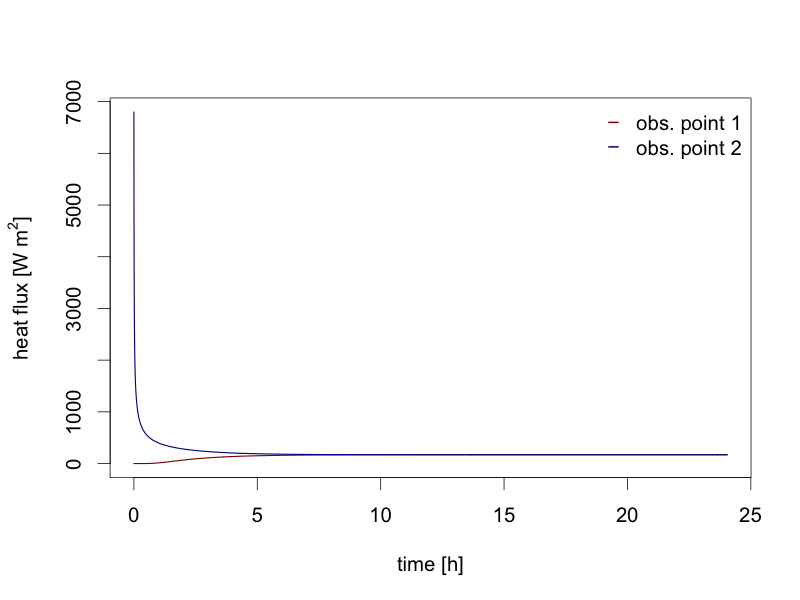
\includegraphics[width=10.5cm]{Fig_heat1/obs_point_temp_sandstone.png}
\caption{\label{plot5} Heat flux at observation points 1 and 2 for sandstone generated with Rscript heatplots.R}
\end{figure}


\subsection*{Question 3}
Heat conduction through a 20 cm thick cotton fibre wall. 

The cumulative heat flux after 24 h at observation point 2 in sandstone is higher than in concrete stone, namely 5014 W m$^{-2}$. With a wall area of 15 m$^2$ this results in $Q = 5014~\mathrm{W~h~m^{-2}}\cdot~15~\mathrm{m^{2}}= 75210 ~\mathrm{W~h}$. 
For the next 24 h, the heat flux will be constant at 170 $\mathrm{~W~m^{-2}}$. The total heat loss will therefore also be $Q=170 \mathrm{~W~m^{-2}}~\cdot 24~\mathrm{h}~\cdot~15~\mathrm{m^{2}}=61200 \mathrm{~W~h}$.

\begin{figure}[!h]
\centering
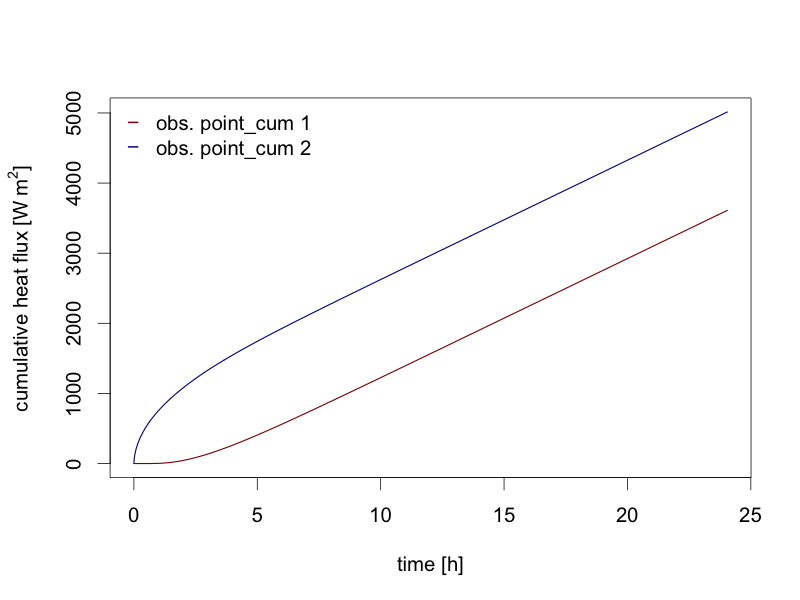
\includegraphics[width=10.5cm]{Fig_heat1/obs_point_cum_temp_sandstone.png}
\caption{\label{plot6} Cumulated heat flux at observation points 1 and 2 for sandstone generated with Rscript heatplots.R}
\end{figure}

\newpage
\newpage
\newpage
\clearpage
\section*{Scenario 3}

\begin{enumerate}
\item Open \emph{heat.conf} in a text editor of your choice. 
\item Change the specific heat capacity and thermal conductivity with values of cotton.
\item Save heat.conf.
\end{enumerate}

\section*{Run scenario 3}
Run the simulation in the terminal console.
\begin{enumerate}
\item Make sure you are in the right directory. 
\item To execute $DRUtES$: \\
\$ bin/drutes
\item After the simulation finishes, to generate png plots execute provided R script: \\
\$ Rscript drutes.conf/heat/heatplots.R cotton
\item The output of the simulation can be found in the folder out
\end{enumerate}

\section*{Tasks for scenario 3}

\begin{enumerate}
\item Answer the same questions as for scenario 1. What is different to scenario 1 and 2?
\end{enumerate}

\section*{Result of scenario 3}
\subsection*{Question 1}
In contrary to scenario 1 and 2, figure \ref{plot7} and \ref{plot8} show that we have not reached steady-state within 24 h. This is because of the very low thermal heat conductivity of cotton fibre. 

\begin{figure}[!h]
\centering
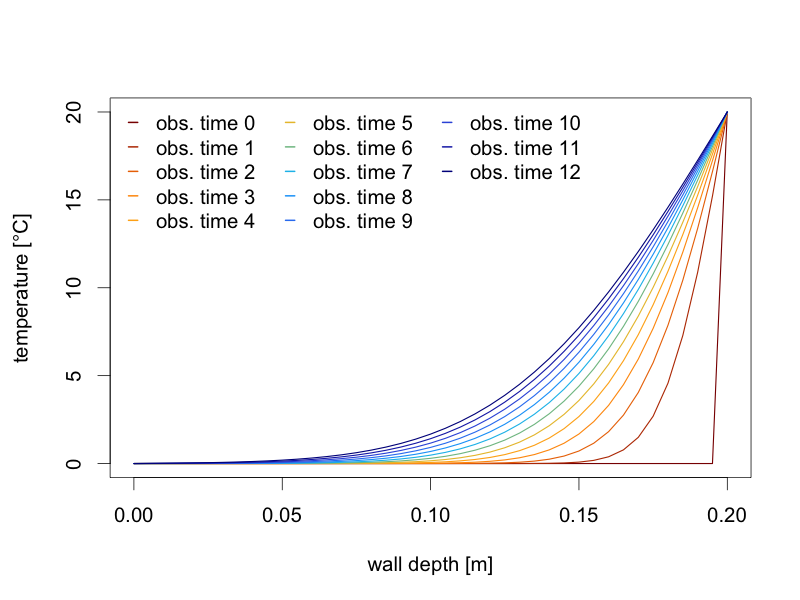
\includegraphics[width=10.5cm]{Fig_heat1/obs_time_temp_cotton.png}
\caption{\label{plot7}Plot of observation times for cotton generated with Rscript heatplots.R}
\end{figure}

\subsection*{Question 2}

\begin{figure}[!h]
\centering
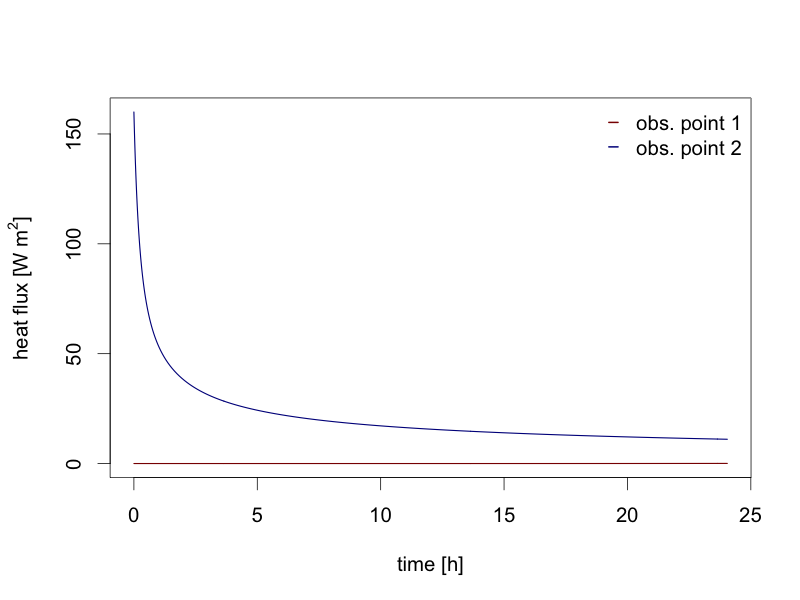
\includegraphics[width=10.5cm]{Fig_heat1/obs_point_temp_cotton.png}
\caption{\label{plot8} Heat flux at observation points 1 and 2 for cotton generated with Rscript heatplots.R}
\end{figure}

We cannot estimate the constant heat flux during steady-state with our results. Using the heat flux equation mentioned during scenario 1, we can calculate the heat flux during steady state:
\begin{equation*}
\phi_{\mathrm{p}}=-\lambda\frac{dT}{dx}= -0.04 \frac{20-0}{0.2}= 4 \mathrm{~W~m^{-2}}
\end{equation*}

\subsection*{Question 3}

The cumulative heat flux after 24 h at observation point 2 in sandstone is higher than in concrete stone, namely 503 W m$^{-2}$, so about a tenth of sandstone and stone concrete. With a wall area of 15 m$^2$ this results in $Q = 503~\mathrm{W~h~m^{-2}}\cdot~15~\mathrm{m^{2}}= 7545 ~\mathrm{W~h}$. 

Since the system is not in steady state, it is difficult to estimate the heat loss for the next 24 h. The answer has to be evaluated numerically by increasing the end time to 48 h. 

\begin{figure}[!h]
\centering
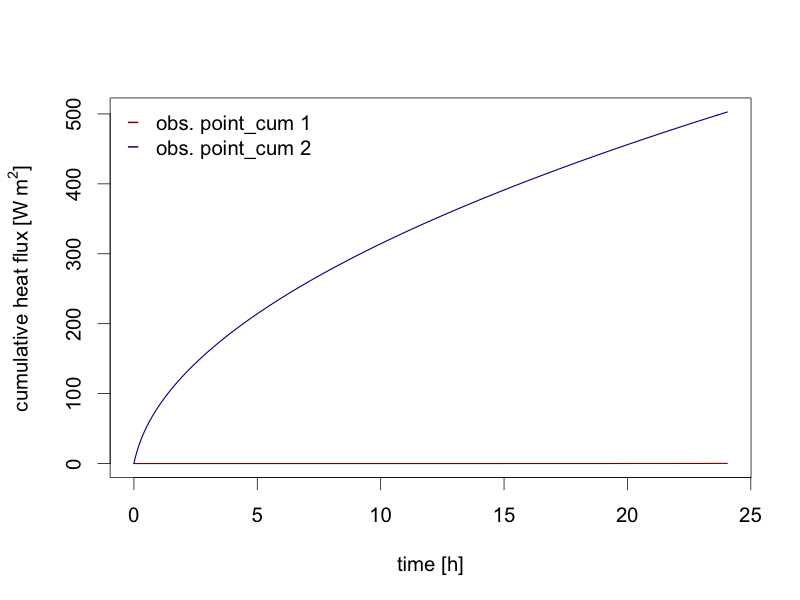
\includegraphics[width=10.5cm]{Fig_heat1/obs_point_cum_temp_cotton.png}
\caption{\label{plot9} Cumulated heat flux at observation points 1 and 2 for sandstone generated with Rscript heatplots.R}
\end{figure}

\newpage
\newpage

\subsection{Outcome}
\begin{enumerate}
\item You got familiar with the $DRUtES$ heat module in 1D.
\item You simulated heat conduction through a wall with different materials
\item You understand the effects of different heat capacities and thermal conductivities.
\item You understand the terms \emph{Dirichlet boundary condition}, \emph{initial condition} and \emph{steady state}.
\end{enumerate}
